\section{User-Authentication}

\subsection{Registrieren eines neuen Nutzers}

Für die Registrierung eines neuen Nutzers müssen seine E-Mail-Adresse inklusive seines 
gewählten Passwords sowie seine Zustimmung zur an die API gesendet werden. 

Dies geschieht über die Form im Signup-Screen.

\begin{code}
    \centering
    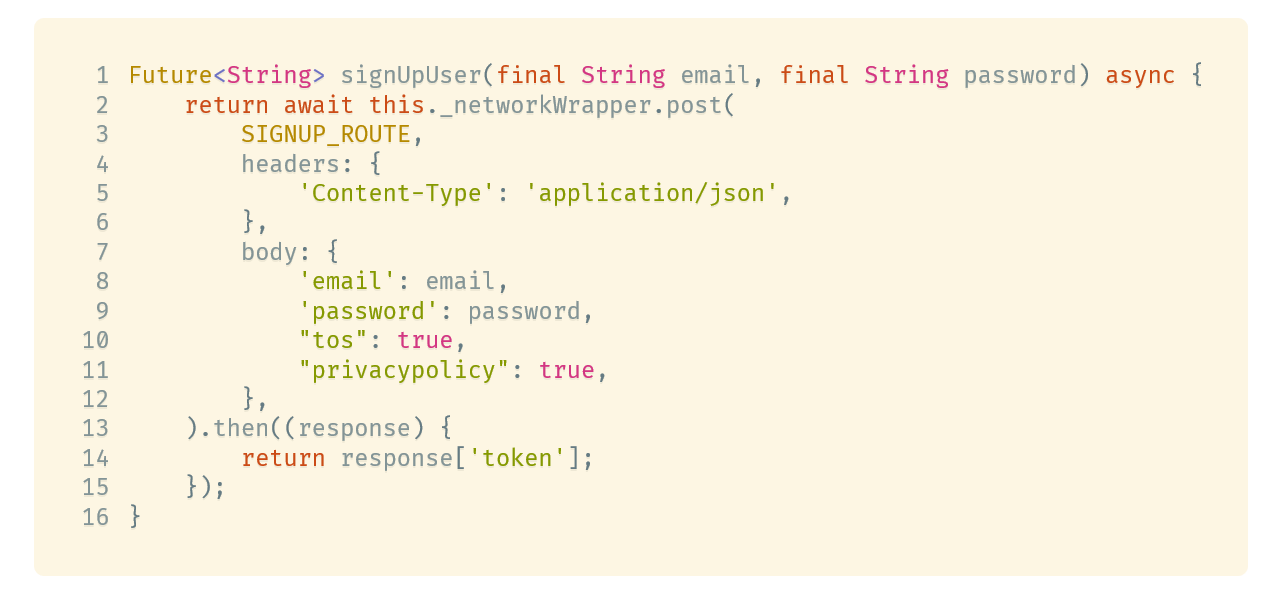
\includegraphics[width=1\textwidth]{images/Dart/services/user-auth/signup.png}
    \caption{Funktion zum Registrieren eines neuen Nutzers}
\end{code}

Ist der Request erfolgreich, so wird ein neuer Nutzer in der Datenbank erzeugt. Als Antwort wird der
Token für die damit generierte Nutzer-Session übermittelt, welcher in weiterer Folge im CookieStorage
abgespeichert wird.

\newpage

\subsection{Anmelden eines vorhandenen Nutzers}

Zur Anmeldung eines bestehenden Nutzers in der App müssen dessen Logindaten an die 
\lstinline{/user/login}-Route der Sokka-API gesendet werden.\\

\begin{code}
    \centering
    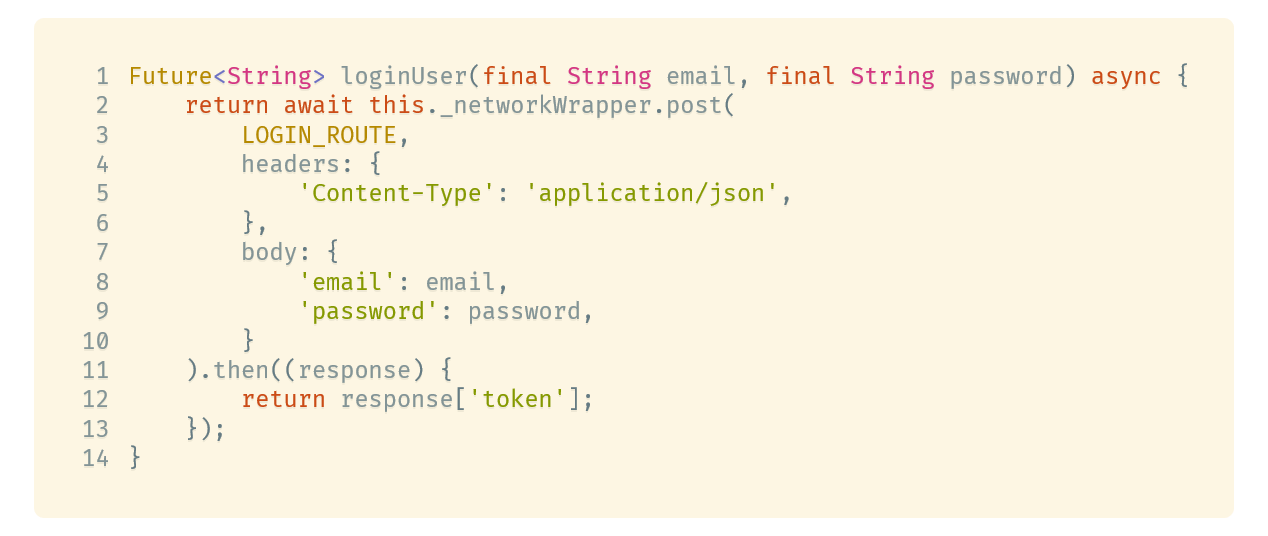
\includegraphics[width=1\textwidth]{images/Dart/services/user-auth/login.png}
    \caption{Funktion zum Anmelden eines bestehenden Nutzers}
\end{code}

\subsection{Abmelden eines Nutzers}

Wenn sich ein Nutzers manuell in der App abmeldet wird ein Request an \lstinline{/user/logout} mit
dem gespeicherten Session-Token und der E-Mail des Nutzers gesendet.

Jener Session-Token wird in weiterer Folge ungültig gemacht und aus dem Cookie-Storage der App
gelöscht, wodruch der Nutzer beim nächsten App-Start wieder zum Login-Screen weitergeleitet wird.

\begin{lstlisting}
Future<void> logoutUser(final String sessionToken, final String email) async {
    await this._networkWrapper.post(
        LOGOUT_ROUTE,
        headers: {
            'Content-Type': 'application/json',
        },
        body: {
            'token': sessionToken,
            'email': email
        },
    );
}
\end{lstlisting}

\subsection{Validieren einer Nutzer-Session}

Damit sich ein Nutzer der Sokka-App nicht bei jedem Start der App mit seinen Logindaten neu
anmelden muss, werden die E-Mail-Adresse und der Session-Token nach einer erfolgreichen Anmeldung
im CookieStorage abgespeichert.

Mit jenen Daten im Speicher kann nun bei jedem weiteren App-Start ein Request an die
\lstinline{/user/validate}-Route mit Session-Token und E-Mail zur Validierung der Nutzer-Session
gesendet werden.\\
Wenn der Session-Token nachwievor gültig ist wird der Nutzer automatisch zum Home-Screen weitergeleitet.
Ist die Session abgelaufen erscheint der Login- bzw. Signup-Screen.

\begin{lstlisting}
Future<bool> validateSessionToken(final String sessionToken, final String email) async {
    return await this._networkWrapper.post(
        VALIDATE_ROUTE,
        headers: {
            'Content-Type': 'application/json',
        },
        body: {
            'token': sessionToken,
            'email': email
        },
    ).then((response) {
        return response['success'];
    });
}
\end{lstlisting}

\subsubsection{Wrapper-Methode zur Session-Validierung}

Damit der Check der Validität des gespeicherten Session-Tokens einfach
bei Start der App ausgeführt werden kann gibt es folgende Wrapper-Methode,
die automatisch benötigte Werte aus dem Storage nimmt und einen entsprechenden
Request an die Sokka-API sendet.

\begin{lstlisting}
Future<bool> validateSession() async {
    String email = await this._cookieStorage.getEmail();
    String token = await this._cookieStorage.getSessionToken();

    return await this.validateSessionToken(token, email);
}
\end{lstlisting}